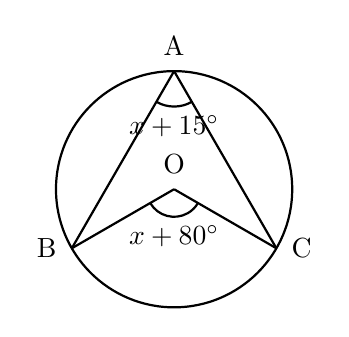
\begin{tikzpicture}[scale=1]

    % Define the center of the circle
    \coordinate (O) at (0,0);

    % Draw the circle
    \draw[thick] (O) circle (1.5);

    % Define points on the circle
    \coordinate (A) at (90:1.5);
    \coordinate (B) at (210:1.5);
    \coordinate (C) at (330:1.5);

    % Draw the lines and segments
    \draw[thick] (A) -- (B);
    \draw[thick] (A) -- (C);
    \draw[thick] (O) -- (B);
    \draw[thick] (O) -- (C);

    % Draw the angle arcs
    % Arc at A (between AB at 240 degrees and AC at 300 degrees)
    \draw[thick] (A) ++(240:0.45) arc (240:300:0.45);
    
    % Arc at O (between OB at 210 degrees and OC at 330 degrees)
    \draw[thick] (O) ++(210:0.35) arc (210:330:0.35);

    % Add labels for the points
    \node[above, yshift=2pt] at (A) {A};
    \node[left, xshift=-2pt] at (B) {B};
    \node[right, xshift=2pt] at (C) {C};
    % Shifted O slightly above to prevent overlapping with the angle text
    \node[above, yshift=2pt] at (O) {O};

    % Add angle values
    \node at (90:0.8) {$x + 15^{\circ}$};
    \node at (270:0.6) {$x + 80^{\circ}$};

\end{tikzpicture}